\documentclass[a4paper, 11pt, oneside]{book}
\usepackage[utf8]{inputenc}
\usepackage{hyperref}
\usepackage{color}
\usepackage{setspace}
\usepackage{geometry}
\newgeometry{left=3.5cm,right=2.5cm,top=2.5cm,bottom=2.5cm}

\usepackage{amsmath}

\makeatletter
\newif\if@restonecol
\makeatother

\let\algorithm\relax
\let\endalgorithm\relax
\usepackage[linesnumbered,ruled,algonl,vlined]{algorithm2e}
\newcommand\mycommentfont[1]{\footnotesize \ttfamily \textcolor{blue}{#1}}
\SetCommentSty{mycommentfont}

\usepackage{graphicx}
\usepackage{epstopdf}
\DeclareGraphicsExtensions{.pdf,.eps,.png,.jpg,.mps}
\usepackage{placeins} % for \FloatbBarrier

\newtheorem{theorem}{Theorem}[section]
\newtheorem{corollary}{Corollary}[theorem]
\newtheorem{lemma}[theorem]{Lemma}

\renewcommand\floatpagefraction{.9}
\renewcommand\topfraction{.9}
\renewcommand\bottomfraction{.9}
\renewcommand\textfraction{.1}

\frenchspacing \sloppy


\newcommand{\eat}[1]{}
\hyphenation{}

\begin{document}

\title{Ensemble Learning in Data Streams}


\author{
Hossain Mahmud \\
Technische Universit\"at M\"unchen\\
mahmud@in.tum.de
}

\date{}

%\maketitle
%\pagenumbering{roman}
%\tableofcontents
%\clearpage
%
%\listoftables
%\addcontentsline{toc}{chapter}{List of Tables}
%\clearpage
%
%\listoffigures
%\addcontentsline{toc}{chapter}{List of Figures}
%\clearpage
%
%\listofalgorithms
%\addcontentsline{toc}{chapter}{List of Algorithms}
%\clearpage

%\normalsize
\onehalfspacing
\pagenumbering{arabic}
\setcounter{page}{1}

\chapter{Related Works}
\label{chp:relworks}
Compared to data mining, stream mining is particularly a very young area. Most of the methods date back only couple of decades. Similarly concept of the ensemble learning was first introduced in the traditional batched learning, however, ensemble adaptations for streams are fairly newer concepts. In this chapter, we list the most influential methods developed so far with particular focus on tree based learners. We follow a rudimentary narrating style starting directly with methods for general stream learners for stationary streams, and then for evolving data. After that, we list the base methods for ensemble learning, and finally presents ensemble based stream learners.

\section{Stream Mining}
Compared to the classical data mining approaches stream mining is relatively a newer topic to be addressed in literature. Even though for batched approaches both classification and clustering problems have been vastly studied, their stream adaption remains a challenge due the restrictions imposed by the stream data. Possibility of temporal locality makes the classification problem harder in a streaming environment. Algorithms needs to address the evolution of underlying data stream. 

Domingos and Hulten introduced a strict one-pass adaptation of decision tree~\cite{breiman84:dt,quinlan93:c45} approach in streams. Classic approaches like ID3 and C4.5 learners assumes that all training examples can be stored in the main memory altogether. This is a significant limitation to the number of examples these algorithms can handle. Similarly, disk based decision tree learners (SLIQ~\cite{mehta96:sliq}, SPRINT~\cite{shafer96:sprint}, etc.) become very expensive when datasets are very large and the expected trees has many levels. Domingos and Hulten proposed \textit{Very Fast Decision Trees (VFDT)}~\cite{domingos00:vfdt} that uses Hoeffding bound~\cite{hoeffding63:bound} to build an anytime decision tree for constant memory and time. The primary assumption in this approach is that, to find the best attribute for a node in a decision tree, it may be sufficient to consider only a fraction of the training set that pass through that node. Hoeffding bound provides an statistical measure to determine how much data is needed to ensure a certain degree of certainty, i.e. error margin would be bounded by a given value~\cite{catlett91:thesis}.

In a recent approach, \cite{rutkowski13:vfdt} argued that using McDiarmid’s bound instead of Hoeffding bound in VFDT is more appropriate for ensuring the approximation bound i.e. the split decisions made after seeing certain number of instances will, with high probability, remain the same for infinite number of instances. The authors also presented McDiarmid’s bound for information gain of ID3 algorithm, and Gini index of CART algorithm. It is to be noted that Hoeffding bound is a special case of McDiarmid’s bound. In another paper, \cite{matuszyk:vfdt} showed usage of Hoeffding bound is mathematically flawed as (i) Hoeffding inequality only applies to arithmetic average, which information gain and Gini index are not, (ii) values obtained in sliding window methods are not independent, while Hoeffding inequality only applies to independent random variables. A revised bound showed that decision bound should be twice of the one given by Hoeffding bound, otherwise, error-likelihood should be updated accordingly.

Like most statistical and machine leaning algorithms VFDT assumes that training data is randomly drawn from a stationary distribution. This assumption is not valid for large databases and data streams. Over time underlying method or environment could change that generates data. The shift is sometimes also referred as {\it concept drift} in literature and can be abrupt as well as very slow. Data related to weather forecast, economic condition prediction, mis-calibrated sensors, etc. are examples of concept drifting environment. A concept-adaptive variant of VFDT, \textit{CVFDT}~\cite{hulten01:cvfdt}, can handle such scenarios. CVFDT updates its decision rules, essentially the tree structure, by detecting the concept drift in the data. It maintains alternate subtrees whenever an old subtree becomes questionable, and replaces the old one with the alternative when it become more accurate. CVFDT uses a sliding window and updates sufficient statistics by increasing the count of newly arrived examples and decreasing the count of old examples in the window. Essentially CVFDT achieves same accuracy that would be achieved if VFDT would have been run again with the new data. CVFDT does this in $O(1)$ with additional space requirement as compared to the VFDT's $O(w)$ where $w$ is the window size. A extension of VFDT, VFDTc was proposed in~\cite{gama05:vfdtc} that improves VFDT by adding continuous numeric attribute handling and naive Bayes prediction at the leaves.

In a different approach to handle concept drift Castillo et al.~\cite{gama03:drift} used Shewhart P-Charts in an online framework based on the idea of \textit{Statistical Quality Control}. Two alternatives of P-charts were used to monitor the stability of one or more quality characteristics in a drifting stream. The two alternatives only differed in the methods they estimate the target value to set the center. The group later introduced another drift detection scheme that monitors probability distribution of examples and maintains a online error rate to detect any concept drift~\cite{gama04:drift}. When distribution changes, error rate will increase. For stationary concept, the error rate should always gradually decrease. A new concept is said to be started if the error rate exceeds some predefined warning or threshold level. This approach has been used in \textit{Ultra Fast Forest Tree (UFFT)}~\cite{gama04:ft, gama05:ft} stream classification method. UFFT maintains naive Bayes statistics for every node. If at any node the error rate starts increasing, the node is pruned for drifting concept. UFFT uses similar approach and Hoeffding bound to control the growth of the tree. For each pair of classes a tree is maintained, hence it is called forest-of-trees.

Another decision tree based approach based on so-called \textit{Peano Count Tree (P-tree)} has been developed by Ding et al. for spatial data streams~\cite{ding02:peanocount}. The Peano Count Tree is a spatial data structure that facilitates a lossless compressed representation of spatial data. This structure is used for fast calculation of information gain for branching in decision trees.

Aggarwal et al. employs a slightly different idea in handling time-evolving data in their on demand classification approach of data streams ~\cite{aggarwal04:ondemand}. They used a modified \textit{micro-clusters concept} introduced in~\cite{aggarwal03:clustream}. Micro-clusters are created from the training data stream only. Each micro-cluster corresponds to a set of points from the training data belonging to the same class. To maintain statistics over different time horizons and avoid storage of unnecessary data points a geometric time frame is used. In the classification task, the \textit{$k$-nearest neighbor} based approach is taken, where micro-clusters are treated as node weighted by their instance counts. 

In~\cite{ganti02:gemm:focus} two algorithms named GEMM and FOCUS have been introduced for streams under block evolution. GEMM is used for model maintenance and FOCUS is for change detection between two data stream models. These algorithms has been tested using decision trees and frequent item set models. FOCUS uses bootstrapping methods to compute the distribution of deviation values when data characteristics remain the same. This distribution is then used to check whether the observed deviation value indicates a significant deviation. In another approach to handle concept drift, Last~\cite{last02:olin} proposed an online classification system OLIN that would dynamically adjust the size of the training window and the number of new examples between model re-constructions to the current rate of concept drift. OLIN uses constant resources to produce models, and achieves nearly the same accuracy as the ones that would be produced by periodically re-constructing the model from all accumulated instances.

Later, Aggarwal proposed an concept drift technique based on velocity density estimation \cite{aggarwal03:condrift}. Velocity density estimation is a technique to understand, visualize, and determine trends in the evolving data. The work presented a scheme to use velocity density estimation to create temporal velocity profiles and spatial velocity profiles at periodic instants in time. These profiles are then used to predict dissolution, coagulation, and shift in data. Proposed method could detect changes in trends in a single scan with linear order of number of data points. Additionally a batch processing techniques to identify combinations of dimensions which results the greatest amount of global evolution are also introduced. In~\cite{kifer04:condrift} authors tried to formally define and quantify the change so that existing algorithms can precisely specify when and how the underlying distribution has changed. They employed a two fixed-length window model, where a current one is updated every time a new example arrives and a reference one is only updated when a change has been detected. To compare the distributions of the windows $L1$ distance has been used [confirm!read again]. Another method to compare two distribution has been presented in~\cite{dasu05:condrift} where authors used Kullback-Leibler (KL) distance to compare two distributions. KL distance is known to be related to the optimal error in determining the similarity of two distributions. In this non-parametric method no assumptions on the underlying distributions is required. 

% TODO: briefly include multi-label evolving ...
% TODO: frequent item set mining]

\section{Ensemble Learning}
Traditional machine learning algorithms generally feature a single model or classifier such as \textit{Na\"ive Bayes} or \textit{Multilayer Perceptron (MLP)}. The free parameters of these learners (e.g. weights of feed-forward neural network) are set by realizing the complete training set. These classifier provides a measurement of the generalization performance i.e. how well the classifier generalizes the training set. However, given a finite set of training example, it is rather reasonable to assume that the data might contain several different generalization. For example, a different setting of neural network classifier (weights, node layers, node counts, etc.) changes the final network to some extent. For stream environment, this assumption becomes primitive. Thus, choosing a single classifier is not always optimal. Using the best classifier among several classifiers where each are trained with same training set would be an alternative, however, information is still being lost by discarding sub-optimal options. A better alternative would be to build a classifier ensemble. Ensemble classifiers combine the prediction of multiple base level model built on traditional algorithm. A simple process for combining prediction could be to choose the decision based on majority voting~\cite{parhami94:voting}. As demonstrated in several works~\cite{breiman93:regression, schapire90:whyens, wolpert92:whyens} ensemble methods (e.g. ensembles of neural networks)~\cite{hansen90:ensNN, tumer99:whyens} yield better performance. 

Without proper selection and control over the training process of the base learners, ensemble classifiers could result in poorer performance. Simply choosing a base classifier and training it for several settings would surely produce highly correlated classifiers which would have adverse effect on the ensemble process. One solution of this issue is to train each classifier with its own training set generated by sampling the original one. However, with random sampling each classifier would receive a reduced number of training patterns, resulting a reduction in the accuracy of the individual base classifier. This reduction in the base classifier accuracy is generally not recovered by the gain of combining the classifier unless measures are taken to make the base classifiers \textit{diverse}. Classifiers with complementary information would give the lowest correlation~\cite{breiman93:regression, tumer99:whyens}. Many methods have been proposed to promote diversity among the base classifier: \textit{bagging}~\cite{breiman94:bagging}, \textit{boosting}~\cite{drucker94:boosting, freund97:boosting, oza99:whyens}, \textit{cross-validation partitioning}~\cite{krogh95:ensNNcv, tumer99:whyens}, etc. These methods mainly process the entire training set repeatedly and require at least one pass for each base model. This is not suitable for streaming scenarios. Stream adaptation of bagging and boosting methods has been introduced by Oza et al.~\cite{oza01:obagboost,oza01:thesis}.

\subsection{Ensemble Learning in Streams}
Learning algorithms in data streams require maintenance of a hypothesis based on the training instances seen thus far with the need for storage and reprocessing. Facilitating this requirement, Oza and Russell developed an online version~\cite{oza01:obagboost, oza01:thesis} of traditional bagging and boosting. Bagging works by randomly sampling with replacement from the training set to form a given number of intermediate training sets which are used to train same number of classifiers. During testing a majority voting scheme is employed on the decisions of all classifiers to deduce the final decision. Boosting uses an iterative procedure to adaptively change distribution of training data by focusing more precisely on misclassified instances. Initially all instances have equal weights, and at the end of a boosting round weight of each instance is updated by increasing or decreasing if the instance was classified wrongly or correctly, respectively. For \textit{online} variant of these algorithms, not knowing the size of the training data poses a problem in determining the size of training sets to build the base models. In~\cite{oza01:obagboost} authors address this situation by training $k$ models with each instances where $k$ is a suitable Poisson random variable. Later on,~\cite{pelossof08:boosting} proposed the \textit{Online Coordinate Boosting} algorithm where the number of weight updates of~\cite{oza01:obagboost} is reduced using few simple alteration.

Online bagging and boosting method do not particularly give attention to the concept drifting nature in the data. \textit{Accuracy Weighted Ensemble (AWE)}~\cite{wang03:accuweighted} is one of the earliest work on concept-drifting stream data. AWE assumes that the stream is delivered in chunks of defined size. With each incoming chunk, AWE updates its $k$ classifiers. Each classifier is associated a weight which is inversely proportional to the expected error of the respective classifier. To estimate this error, it is assumed that the distribution of test set is closest to the most recent chunks. Concept drift is adapted by effectively manipulating the number and the magnitude of the weights that are changing. An extension of AWE has been proposed in~\cite{brzezinski11:accuupdated}, namely \textit{Accuracy Updated Ensemble (AUE)}. AUE takes the weighting motivation from AWE, but improves the limitation of AWE. In AWE each classifier learns from the incoming chunks in a ``batched'' fashion. AUE employs an online scheme instead. AUE also adapts the weighting function to reduce the adverse effect in AWE of sudden drift in data. AWE weighting function is prone to suffer by rapid change in the stream and most or even all classifiers assuming they are ``risky''. This limitation has been addressed in AUE. Result shows that AUE performs marginally better than AWE, however, also requires slightly longer time and larger space.

As mentioned in the previous section, \textit{Hoeffding Tree (HT)} i.e. VFDT~\cite{domingos00:vfdt}, can be used to build classifiers for concept drifting streams. The Hoeffding Tree has the property that it adapts itself for the newer examples. The number of examples that a HT is build upon is determined by two numbers: (i) the be size of the tree, and (ii) the number of examples used to create a node. Thus, smaller trees adapt faster to the changes in the data, while larger trees tries to retain the rules that reflect longer time-frame, simply because they are built on more data. In other words tree bounded by size n would be reset twice as often as tree bounded by size $2n$. \textit{Adaptive Size Hoeffding Tree (ASHT)}~\cite{bifet09:asht} uses this intuition to build an ensemble of classifiers of different sized Hoeffding trees. ASHT attempts to increase the diversity in the bagging approach. The maximum allowed size for $n$-th tree is twice the size of $(n-1)$-th, where the 1st tree has a size of $2$. Additionally inverse of the squared error has been used as the weights for the trees. Diversity between the traditional bagging and ASHD bagging are compared using kappa statistic. If two classifier agree on every example then $k = 0$, and if they agree on the predictions purely by chance then $k = 0$. To test this approach authors have used Interleaved Test-then-Train method. At the leaf level of HT, Naive Bayes predictions are used. The experiments were performed on several different generated dataset such as SEA Concepts Generator, STAGGER Concepts Generator, Rotating Hyperplane, Random RBF Generator, etc. Performance are compared with traditional Naive Bayes, HT, and boosting methods. Evaluation concluded that bagging provides best accuracy, however, with the higher cost in terms of running time and memory. Authors made an observation that even bagging using 5 trees of different size might be sufficient for gain higher accuracy, as error level for bagging with 10 trees does not drop much but takes twice time.

Same authors also proposed an adaptive window size bagging method- \textit{ADWIN}~\cite{bifet09:asht}. ADWIN automatically detects and adapts to the current rate of change. To do so ADWIN adapts its window size to maximize the statistically consistently length that conforms following hypothesis ``there has been no change in the average value inside the window''. Window is not maintained explicitly rather using a variant of exponential histogram technique that takes $O(log w)$ memory and $O(log W)$ processing time where $w$ is the length of the window. Experimental evaluation showed that ADWIN has better accuracy than ASHT, however, requires more time and memory. 

ADWIN has later been used in \textit{leverage bagging}~\cite{bifet10:levbag}. Leverage bagging improves randomization by increasing resampling and using output detection codes. Resampling with replacement is done in Online Bagging using Poisson(1). Instead leverage bagging increases the weights of resampling using a larger value $\lambda$ to compute the value of the Poisson distribution. The Poisson distribution is used to model the number of events occurring within a given time interval. In other improvement randomization is added at the output of the ensemble using output codes. Method works by assigning a binary string of length $n$ to each class and building an ensemble of $n$ binary classifiers. Each of the classifiers learns one bit for each position in the string. A new instance is classified to the class whose binary code is closest. 

ADWIN has also been used in building ensemble of \textit{Restricted Hoeffding Trees}~\cite{bifet10:rht}. A mechanism for setting the learning rate of perceptrons using ADWIN's change detection method is used to restrict the tree. Additionally, a mechanism for reseting the member Hoeffding trees is also been introduced when a particular member is no longer performing well. The method outperforms traditional bagging in terms of accuracy, but requires additional memory and time.

Another group of methods known as \textit{random forests} uses bagging of decision trees. The concept of random forest is introduced by Breiman~\cite{breiman99:randomforest}. Random forest works in a similar fashion as bootstrap aggregation. However, for each split in the tree it only selects a subset of the features to be considered for splitting criterion. This \textit{feature bagging} approach helps avoiding very strong predictors to get selected over and over. One method mentioned before, \textit{Ultra Fast Forest Tree (UFFT)}~\cite{gama04:ft, gama05:ft} uses concepts of tree bagging, however, works with all features the whole time. UFFT maintains statistical information on each node to detect drift and grows the tree in a similar  approach to VFDT. Using the statistical information stored in nodes it detects concept drift with naive Bayes error-rate. Abdulsalam et al. proposed \textit{Dynamic Streaming Random Forests (DSRF)} focusing on lowering the number of examples required to build up new model in a drifting environment~\cite{salam08:dsrf, salam11:dsrf}. Shannon entropy~\cite{shannon01:entropy} is used to detect concept drift. All these methods are empirically proven to be effective for generalized scenario and chosen data sets. 



\chapter{Background}
\label{chp:background}
This chapter discusses the primitives of data and stream classification. First, a brief overview of traditional data classification methods are presented. Followed by a section on data stream classification where challenges and approaches for stream classification are introduces. Finally, overview of current state-of-the-art ensemble learning methods are discussed. These discussion are lays the foundation of the approach introduced in this thesis.


\section{Learning Algorithms}
The goal of data classification process is to predict a certain outcome based on some give data. In order to do so, data mining algorithms first processes a training set containing a set of attributes and corresponding outcome: a class or value. Algorithms develop hypotheses that best describe the relationship among the attributes and the outcome for the total instance set. 
Formally, learning are defined as follow: Given a data set of m instances 
$D \equiv \{ \{\vec{x}_1, y_1\}, \{\vec{x}_2, y_2\}, \{\vec{x}_3, y_3\}, \dots, \{\vec{x}_m, y_m\} \}$ 
for $i = \{ 1, 2, 3, \dots, m \}$ and $ \vec{x} = \{x_1, x_2, x_3, \dots, x_n\}$, 
learning algorithms try to approximate $H \equiv y = f(\vec{x})$. 
Additional to being typical linear, polynomial, etc. functions, $H$ can also be a set of IF-THEN rules. 
These rules or functions are then used to predict unseen instances where outcome class is not known. These algorithms are known as learning algorithms, and in last few decades, have widely been researched in the field of machine learning. This section briefly discusses few of the basic algorithms upon which the foundation of ensemble methods and this thesis is laid. 

\subsection{$k$-Nearest Neighbors}
\begin{figure*}[htbp]
    \begin{center}
        \includegraphics[width=3.0in]{figs/knn.jpg}
        \caption{Concept of $k$-NN.}
        \label{fig:bg:knn}
    \end{center}
\end{figure*}

\subsection{Na\"ive Bayes}
Naive Bayes classification is based on Bayes rule. Bayes rule says that the probability of event $x$ conditioned on knowing event $y$, i.e. the probability of $x$ given $y$ is defined as
\[
    p(x|y) = \frac{p(x,y)}{p(y)} = \frac{p(y|x) p(x)}{p(y)}
\]
The naive Bayes classifier~\cite{langley92:nb} assumes that all the explanatory variables are independent. Given a feature set $X = x_1, x_2, \dots, x_n$ of $n$ independent variables, naive Bayes assigns the instances to $k$ possible outcome or classes, $p(C_k | X)$. Using Bayes rule, the conditional probability can be decomposed as
\[
    p(C_k |X) = \frac{p(C_k) p(X|C_k)}{p(X)}
\]
In other words,
\[
    posterior = \frac{prior \times likelihood}{evidence}.
\]
Using chain rule repetitively, it can be expressed as follows:
\[
    p(C_k |X) = p(C_k) \prod_{i=1}^n p(x_i | C_k)
\]
The predicted class is the one which maximizes the conditional probabilities $p(C_k|X)$, that is, classifier assigns the class label $\hat{y} = C_k$ for some $k$ that satisfies:
\[
    \hat{y} = \underset{k \in \{1, \dots, K\}}{argmax}  p(C_k) \prod_{i=1}^n p(x_i | C_k)
\]

\subsection{Decision Tree}
Decision trees are another popular genre of non-parametric supervised learning algorithms. Trees allow a way to graphically organize a sequential decision process. Decision tree, a directed acyclic graph, contains decision nodes, each with branches for all alternate decisions. Leaf nodes are labeled with respective class label. Each path from root to leaf is a decision rule, consisting of conditional part (unions of all internal nodes' conditions) and a decision (of leaf node).

Decision trees use {\it information gain} to select the splitting attribute that would maximize the total entropy of each of the subtrees resulting from the spit. Entropy is a measurement of purity of an attribute, typically ranged between 0 and 1. A pure attribute, attribute with definitive value-class relationship, would have a low entropy and is easy to predict. On the other hand attribute with highly mixed value-class relationship would yield high entropy. A common entropy function is-
\[
    entropy = - \sum_{i=1}^n p_i \lg p_i.
\]
where $p_1, p_2, \dots, p_n$ are the distributions of several class attributes and $\sum p_i = 1$. Information gain is the difference between old and new entropy after a split. This is good measurement of relevance of an attribute. However, in cases where an attribute can take on a large number of distinct values, information gain is not ideal. Presence of large set of values could uniquely identify the classes but also reduces chance to generalize unseen instance and should be avoided to be place near root.

Decision tree is, however, computationally feasible. Average cost of constructing a decision tree for $n$ instances with $m$ attributes is $O(mn \lg n)$, and querying time is $O(\lg n)$.

\subsection{Neural Network}

\section{Data Stream Classification}
Traditional data mining algorithms work in a memory bounded environment and requires multiple scan of the training data. In stream environment, one of the major assumptions is that new data samples are introduced in the system with such a high rate that repetitive analysis becomes infeasible. Thus, for stream classification, algorithms should be able to look into a instance only once and decide upon that. A bounded memory buffer can be used to facilitate some level of repetition. However, which instances are to remember and which are to forget would then become a decision choice. An alternate choice is to maintain sufficient statistics to have a representation of the data. The process of deletion or summarization of instances, however, means that some information are being lost over the time.

In this section, these challenges are first discussed in details. Then it presents the basis of some of the concepts arisen to handle these challenges. Finally, before moving onto the ensemble leaning, it discusses current state-of-the-art algorithms for stream mining.

\subsection{Challenges}
Challenges posed by the streaming environment can be categorized into two groups: (i) relating to runtime and memory requirements and (ii) relating to underlying concept identification. Speed of incoming data, unbounded memory requirement, single-pass learning fall into the first category. On the other hand, lack of labeled data, concept drifting, evolution and recurrence are examples of latter category.

\paragraph{Speed of data arrival}
As mentioned before, it is an inherent characteristic of data streams that it arrives with a high speed. The algorithm should be able to adapt to the high speed nature of streaming information. The rate of building the classifier model should be higher than the data rate. This gives a very limited amount of available time for classification as compared to the traditional batch classification models.

\paragraph{Memory requirements:}
To apply traditional batched approaches in streaming data, an unbounded memory would be needed. This challenge has been addressed using load shedding, sampling, aggregation, etc. Rather than storing all the instances, algorithms store a subset of the data set or some statistical values or a combination of both which represents the data seen thus far. New instances can be classified only by looking into these stored information. 

\paragraph{Single-pass learning:}
The premise of this requirement is two-fold. First, as mentioned above, data would not be available in the memory after a short period of time due to the volume of data. Secondly, even if the data remain available, running a batched-like approach for millions of data points would highly increase the running time of the algorithm. To attain faster processing time with limited storage, algorithm should access the data stream only once, or a small number of times. Mining models must posses the capability to learn the underlying nature of data in a single pass over the data.

\paragraph{Lack of labeled data:}
Unlike most data sets or settings of batched approaches, steam mining data sets are often poorly labeled. A large number of experimentations are done with generated data set where the data generation process can easily be controlled to have proper labeling. However, in data set collected from real world are often lack this. For example, to setup a supervised learning experimentation using a data set collected from social media, e.g. Twitter, data needs to be first categorized by human intervention. Manual labeling of such data is often costly, both in terms of resources and time. In practice, only a small fraction of data is labeled by human experts or automated scripts. A stream classification algorithm is thus required to be able to predict after observing a small number of instances, i.e. to be ready to predict anytime.

\begin{figure*}[htbp] 
    \begin{center}
        \begin{tabular}{cc}
            \resizebox{60mm}{!}{\includegraphics{figs/condrift-a.jpg}} &
            \resizebox{60mm}{!}{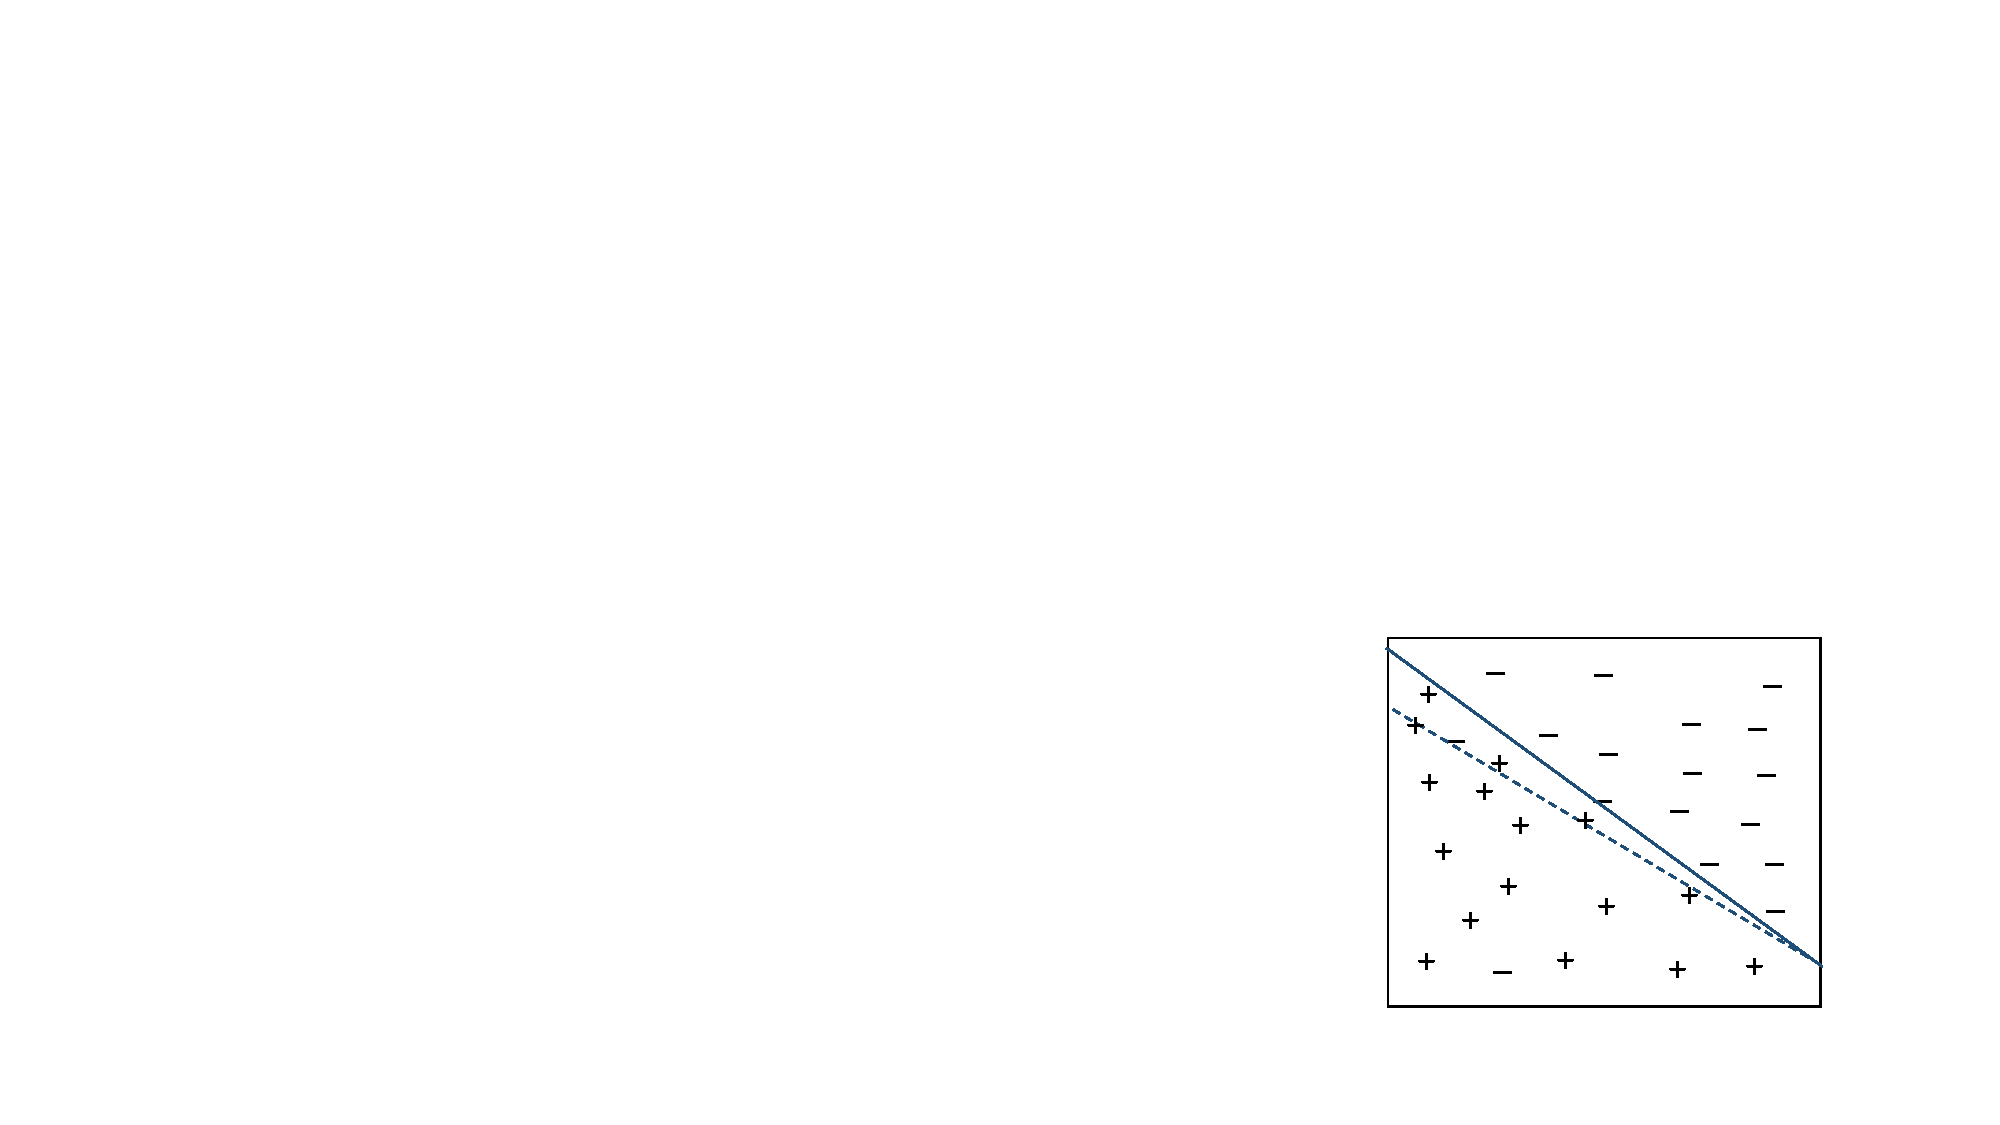
\includegraphics{figs/condrift-b.jpg}} \\
            \scriptsize{(a)\hspace{0mm}} & \scriptsize{(b)}    
        \end{tabular}
    \caption{Concept drift in data streams.}
    \label{fig:bg:condrift}
    \end{center}
\end{figure*}
\paragraph{Concept drift:}
Concept drift is a statistical property of data streams where the target variable drifts away from the model that is trying to predict it. In other words the underlying data distribution is changing over time. As a result accuracy of the classifier model decreases over time. For example, buying pattern of the customers in a store changes over time, mostly due to the seasonality. Electrical and mechanical devices wear off over time, producing shifted result which would cause drift in the observing data. Learning models should adapt to these changes quickly and accurately. Let us consider the example in Figure~\ref{fig:bg:condrift}. As a new chunk arrives (Figure~\ref{fig:bg:condrift}a), a new classifier is learned. The decision boundary is denoted by the straight line. The positive examples are represented by unfilled circles while the negative examples are represented by filled circles. With time the concept of some of the examples may change. As shown in Figure~\ref{fig:bg:condrift}b, due to concept drift some negative examples may have become positive. So, the previous decision boundary has become outdated and a new model has to be learned. Formally, concept drift is the change in the joint probability \(P(X, y) = P(y|X) \times P(X)\). Thus, observing the change in $y$ for given $X$, i.e. $P(y|X)$ is the key for detection.

One challenge posed here is to differentiate the noise in data and the actual shift of the concept. Often in streaming environment data contains the both. Rate of drift is also a factor in detection. Sudden drift, known as {\it concept shift}, is easier to detect than concept drift, which is considered to be gradual.

\begin{figure*}[htbp]
    \begin{center}
        \begin{tabular}{cc}
            \resizebox{60mm}{!}{\includegraphics{figs/conevol-a.jpg}} &
            \resizebox{60mm}{!}{\includegraphics{figs/conevol-b.jpg}} \\
            \scriptsize{(a)\hspace{0mm}} & \scriptsize{(b)}    
        \end{tabular}
        \caption{Concept evolution in data streams.}
        \label{fig:bg:dataevol}
    \end{center}
\end{figure*}
\paragraph{Concept evolution:}
Concept evolution is referred to the emergence of a new class or a set of classes in stream data as the time flows. Twitter stream is an ideal example where concept evolution is very easily identifiable. Twitter reacts, seemingly, very fast upon important news around the globe. Looking into the different hash tag usages in such social media currently trending topics can be identified. To present a clearer picture let's consider following example in Figure~\ref{fig:bg:dataevol}. At certain point of time four classes and their corresponding decision boundaries are shown in the Figure~ (\ref{fig:bg:dataevol}a). With the more incoming data a novel class emerges, and for that decision boundaries need updating. Emergence of new class can affect any number of decision boundary/ rule, from one to all.

Concept evolution is also prone to noise. Furthermore, clear distinction between drift and evolution might not always be possible, partially due the lack of unlabeled data.

\paragraph{Class recurrence:}
Class recurrence is a special case of concept drift and evolution. A this case, the model forgets a class due the drift, however, later the class reappears (evolution) from the stream. Seasonality could be one cause of this situation. A intrusion in network traffic may reappear after a long time. Forgetting the earlier intrusions are not desired in such case. A fast recognition of the previously seen classes are desired in mining streams.

Following sections discuss the potential solutions to these challenges. First, how to address the limited resources and then the change detection schemes.

\subsection{Maintaining Sufficient Statistics}
In statistical evaluation, a statistic is sufficient for a family of probability distributions if the sample from which it is calculated gives no additional information than does the statistic, as to which of those probability distributions is that of the population from which the sample was taken~\cite{fisher22:suffstat}. Mathematically, given a set  $\mathbf{X}$ of independent identically distributed data conditioned on an unknown parameter $\theta$, a sufficient statistic is a function $T(\mathbf{X})$ whose value contains all the information needed to compute any estimate of the parameter (e.g. maximum likelihood estimate). Using the factorization theorem (Theorem~\ref{thm:factor}), for a sufficient statistic $T(\mathbf{X})$, the joint distribution can be written as $ p(\mathbf{X}) = h(\mathbf{X}) g(\theta, T(\mathbf{X}))$. From this factorization, it can easily be seen that the maximum likelihood estimate of $\theta$ will interact with $\mathbf{X}$ only through $T(\mathbf{X})$. Typically, the sufficient statistic is a set of function or random variables of the data.

\begin{theorem}[Factorization Theorem]
    \label{thm:factor}
    Let $X_1, X_2, \dots , X_n$ be a random sample with joint density $f(x_1, x_2, \dots , x_n| \theta)$. A statistic $T = r(X_1, X_2, \dots , X_n)$ is sufficient if and only if the joint density can be factored as follows:
    \[
    f(x_1, x_2, \dots , x_n| \theta) = u(x_1, x_2, \dots , x_n) v(r(x_1, x_2, \dots , x_n), \theta)
    \]
    where $u$ and $v$ are non-negative functions. The function $u$ can depend on the full random sample $x_1, x_2, \dots , x_n$, but not on the unknown parameter $\theta$. The function v can depend on $\theta$, but can depend on the random sample only through the value of $r(x_1, x_2, \dots , x_n)$.
\end{theorem}

\subsubsection{Bounds of Random Variable}
A random variable is a variable that can take a set or range of values, each with an associated probability, and are subjected to change due to the alteration or randomness of the data. Random variables are of two types: (i) discrete, and (ii) continuous. Discrete random variable take a set of possible values (e.g. outcome of coin flipping), but a continuous random variable can take any value within a range (e.g. age of people in a randomly sampled group).

A function that is used to estimating a random variable is called an estimator. Estimator function is dependent on the observable sample data, and used for estimating unknown population within an interval with certain degree of confidence. For an interval of the true value of the parameter associates with a confidence of $1 - \delta$, interval can be defined as follows:

\begin{itemize}    
    \item Absolute approximation: $\bar{X} - \epsilon \le \mu \le \bar{X} + \epsilon$, where $\epsilon$ is the absolute error.
    \item Relative approximation: $(1 - \delta)\bar{X} \le \mu \le (1 + \delta)\bar{X}$, where  is the relative error.
\end{itemize}

where $\mu$ and $\bar{X}$ represent actual and estimated mean. There are a number of theorems that provide bounds on the estimation, Chebyshev [!], Chernoff~[!], Hoeffding~\cite{hoeffding63:bound}, etc. are few of them.

\begin{theorem}[Chebyshev]
\label{thm:chebyshev}
    Let $X$ be a random variable with standard deviation $\sigma$, the probability that the outcome of $X$ is no less than $k\sigma$ away from its mean is no more that $1/k^2$:
    \[
        P(|X-\mu| \le k\sigma) \le \frac{1}{k^2}
    \]
    In other words, it states that no more that $1/4$ of the values are more than $2$ standard deviation away, no more than $1/9$ are more than $3$ standard deviation away, and so on.
\end{theorem}

\begin{theorem}[Chernoff Bound]
\label{thm:chernoff}
    Let $X_1,X_2,\dots, X_n$ be independent random variables from Bernoulli experiments. Assuming that $P(X_i = 1) = p_i$. Let $X_s = P_n \sum_{i=1}{n} X_i$ be a random variable with expected value $\mu_s = P \sum_{i=1} np_i$. Then for any $\delta > 0$:
    \[
        P[X_s > (1+\delta) \mu_s] \le (\frac{e^\delta}{(1 + \delta)^{1 +\delta}} )  ^{\mu_s}
    \]
    and the absolute error is:
    \[
        \epsilon \le \sqrt{\frac{3 \bar{\mu}}{n} \ln (2/\delta)}
    \]
\end{theorem}

\begin{theorem}[Hoeffding Bound]
\label{thm:hoeffding}
    Let $X_1,X_2,\dots, X_n$ be independent random variables. Assuming that each $x_i$ is bounded, that is $P(X_i \in R = [a_i, b_i]) = 1$. Let $S = 1/n \sum_{i=1}{n} X_i$ whose expected value is $E[S]$. Then, for any $\epsilon > 0$:
    \[
        P[S - E[S] > \epsilon] \le e^{ \frac{2 n^2 \epsilon^2}{R^2} }
    \]
    and the absolute error is:
    \[
        \epsilon \le \sqrt{\frac{R^2 \ln(2/\delta)}{2n}}
    \]
\end{theorem}

Chernoff and Hoeffding bounds are independent of the underlying distribution of examples. They are more restrictive or conservative, and requires more observations as compared to the distribution dependent bounds. Chernoff bound is multiplicative and Hoeffding is additive. They are expressed as relative and absolute approximation, respectively.

These methods only take a finite number of values or a range. One of the well-known methods supports infinity is Poisson process. A random variable $x$ is Poisson random variable with parameter $\lambda$ if $x$ takes values $0,1,2, \dots, \infty$ with:
    \[
        p_k = P(x=k) = e^{-\lambda} \frac{\lambda^k}{k!}
    \]
    where, $\lambda$ is both mean and variance, i.e. $E(X) = Var(X) = \lambda$
    
\subsubsection{Recursive Mean, Variance, and Correlation}
Fundamental equation of mean, variance, etc. are not usable for streams as past data points are lost as the time passes. However, their recursive version are also known. Equation~\ref{eqn:mean}, \ref{eqn:var}, and \ref{eqn:corr} can be used to recursively compute mean, variance, and correlation respectively.

\begin{equation}
\label{eqn:mean}
    \bar{x}_i = \frac{(i-1) \times \bar{x}_{i-1} + x_i}{i}
\end{equation}

\begin{equation}
\label{eqn:var}
    \sigma_i = \sqrt{ \frac{\sum x_i^2 - \frac{ (\sum x_i )^2}{i} }{i-1} }
\end{equation}

\begin{equation}
\label{eqn:corr}
    corr(a, b) = \frac{ \sum(x_i \times y_i) - \frac{\sum x_i \times \sum y_i}{n} }{\sqrt{\sum x_i^2 - \frac{\sum x_i^2}{n}} \sqrt{\sum y_i^2 - \frac{\sum y_i^2}{n}}}
\end{equation}

As it can be seen from the equations, maintaining (i) number of observations, $n$; (ii) $\sum x_i$, sum of $i$ data points; (iii) $\sum x_i^2$, sum of squares of $i$ data points; and (iv) $\sum (x_i \times y_i)$, sum of cross product of $X$ and $Y$ are enough to recursively compute these statistics.


\subsubsection{Windowing}
Windowing the process of selecting a subset of the observed instances that would be remembered to be used in the computation of statistics. Where the data set is finite and of limited size, all the instances can be remembered. For streams, this is not possible. Furthermore, computing statistics over all the instances of the past, in streaming environment would wrongly introduce information of classes that are not needed in the present. Thus, information of recent past is more important than the entire set. Windowing is categorized in two basic types: (i) sequence based windowing, and (ii) time-stamp based windowing.

In sequence based windowing, sequence is based on the number of observations seen; in time-stamp based approach, it is elapsed time. Landmark windowing and sliding windowing are two most used sequence based windowing system.

\paragraph{Landmark Windowing:} All observations after certain start point are remembered. Batched approaches can be thought of as examples of landmark windowing where every instance is remembered from the very first one. As new observations are seen, size of window increases. Landmark needs updating time to time to ensure recency of the statistics.

\paragraph{Sliding Windowing:} A fixed length window is moved through the observation set. As a new observation is seen, oldest observation is forgotten, i.e., when $j$-th instance is pushed into the window, $(j-w)$-th instance is forgotten, where $w$ is the size of the window. A limitation of sliding windowing is that it requires all elements within the window to be remembered, as it is needed to forget the oldest observation.

Often it is more useful to learn about most recent updates with fine granularity and older ones in a summarized fashion. With this motivation concept of tilted-time windowing was introduced~\cite{chen02:tiltedtime}.

\begin{figure*}[htbp]
    \begin{center}
        \includegraphics[width=3.0in]{figs/naturaltime.pdf}
        \caption{Natural Tilted Time Window}
        \label{fig:bg:ntime}
    \end{center}
\end{figure*}
\paragraph{Natural Tilted Time Windowing:} In natural tilted time windowing, units of time is distributed non-uniformly. Most recent time gets more units. For example, Figure~\ref{fig:bg:ntime} shows a natural tilted time windowing scheme, where for most recent hour 4 units stores quarterly updates, 24 units of time storing a day, and 31 units storing a months summary. That is, with 59 units of time information, this model stores more than 32 days' information.

\begin{figure*}[htbp]
    \begin{center}
        \includegraphics[width=4.0in]{figs/logtime.pdf}
        \caption{Logarithmic Tilted Time Window}
        \label{fig:bg:ltime}
    \end{center}
\end{figure*}
\paragraph{Logarithmic Tilted Time Windowing:} Concept for logarithmic tilted time windowing is same as natural tilted time windowing. The only deference here is that time scale grows in logarithmic order. Figure~\ref{fig:bg:ltime} shows an example. 


\subsection{Change Detection}
An assumption of most machine learning methods is that data is generated from a stationary distribution. As discussed in the previous section, this assumption does not hold for streaming scenario. Thus stream mining requires algorithms to facilitate drift detection methods. Differentiating between {\it noise} and {\it change} makes the problem challenging. The difference between a new distribution and noise is {\it persistence}, where new examples consistently follows new distribution rather than old. This section discusses several methods to detect and adapt learning algorithms in presence of concept drift.

\subsubsection{Detection}
Detection methods can generally be classified into two categories. First approach is to monitoring the evolution of various performance indicators as done in~\cite{klinkenberg98:changedetection, zeira04:changedetection}. Another approach is to maintaining two (or more) distributions varying the window length. Typically one window would summarize past history while the other would summarize most recent information~\cite{kifer04:condrift}.

Most methods follows the first approach. \cite{klinkenberg98:changedetection} monitors three performance indicators (accuracy, recall, and precision) over time, and uses their posterior comparison to a confident interval of standard sample errors for a moving average value for each indicator.

A classical algorithm for change detection is Cumulative Sum (CUSUM)~\cite{page54:cusum}. CUSUM can detect that the mean of the input data is significantly different than zero. The test is as follows:
\[
    g_0 = 0 
\]\[
    g_t = max (0, g_{t-1} + (r_t - v))
\]
if $g_t > \lambda$ CUSUM triggers an alarm and set $g_t = 0$. This detects the changes in the positive direction, to detect the negative change $min$ is used instead of $max$. CUSUM does not require any memory. Its accuracy depends on the choice of $v$ and $\lambda$. Low $v$ results in faster detection with more false alarms.

For latter category, \cite{kifer04:condrift} uses Cherfnoff bound (Theorem~\ref{thm:chernoff}) and examines examples drawn from two probability distribution and decides whether these distributions are different.

\paragraph{ADWIN Algorithm:} As introduced in previous chapter, ADWIN (ADaptive sliding WINdow) is another change detection algorithm of latter type. ADWIN keeps a variable length window of recent items. It ensures the property {\it there has been no change in the average value inside the window} for maximally statistically consistent length. The core idea of ADWIN is that whenever two {\it large enough} sub-windows of $W$ exhibit {\it distinct enough} averages, it is assumed that their corresponding expected values are different, and the older portion of the window is dropped. Essentially, this means that when the difference of means of the two windows is greater than a certain threshold $\epsilon_{cut}$, the older portion should be dropped. Equation to compute $\epsilon_{cut}$ is as follows:
\[
    m = \frac{2}{1/|W_0| + 1/|W_1|}
\]\[
    \epsilon_{cut} = \sqrt{\frac{1}{2m} \ln \frac{4 |W|}{\delta}}
\]
where $\delta \in (0, 1)$ is confidence value, an input.

\begin{algorithm}[htbp]
    \DontPrintSemicolon
\label{alg:adwin}
\caption{ADWIN Algorithm}

    \KwData{Data Stream}
    \KwResult{Window with most recent concept}
    \Begin{
        Initialize window $W$ \\
        \ForEach{$t > 0$} {
            $W \leftarrow W \cup \{x_t\}$ \tcp*[f]{add $x_t$ to the head of $W$ }\\
            \Repeat{$|\mu_{W_0} - \mu_{W_1}| < \epsilon_{cut}$ holds for every split of $W$} {
                Drop element from the tail of W\\
            }
            $W = W_0 . W_1$\\
        }
        Output $\mu_W$\\
    }
\end{algorithm}

\subsubsection{Adaptation to Change}
To improve accuracy of the decision model under concept drifting environment, decision model needs adaptation to the change. There are two types of approaches based on when to adapt: 
\begin{itemize}    
    \item Blind or Periodic Methods: Models are updated on regular interval whether an changes have actually occurred or not. 
    \item Informed Methods: Models are only updated when there are sufficient reasons to believe that changes in the concept have occurred.
\end{itemize}
It could a good idea to use periodic methods where duration of seasonality is known beforehand. Otherwise, chosen duration could be too large or too small to response to the change. In such cases, an informed decision is more desired. However, informed methods requires more resources (than blind methods) to be able to make such decision.


\subsection{Na\"ive Bayes Adaptation}
Naive Bayes algorithm is essentially a stream classification algorithm. One of the advantages of this classifier in the context of data stream is its low complexity for deployment. It only depends on the number of explanatory variables. Its memory consumption is also low since it requires only one conditional probability density estimation per variable.

\subsection{Very Fast Decision Tree}

\begin{algorithm}[htbp]
    \DontPrintSemicolon
\SetKwInOut{Input}{Input} \SetKwInOut{Output}{Output} 
\label{alg:vfdt}
\caption{VFDT: The Hoeffding Tree Algorithm}

    \Input{$S$: Stream of examples \\
           $X$: Set of nominal attributes \\
           $Y$: Set of class labels $Y = \{y_1, y_2, \dots, y_k\}$ \\
           $G(.)$: Split evaluation function \\
           $N_{min}$: Minimum number of examples \\
           $\delta$: is one minus the desired probability \\
           $\tau$: Constant to resolve ties
          } 
    \Output{$HT$: is a decision tree}
    
    \Begin{
        Let $HT \leftarrow$ Empty Leaf (Root)
        \ForEach{$example(x, y_k) \in S$} {
            Traverse the tree $HT$ from root till a leaf $l$ \\
            
            \eIf (\tcp*[f]{Missing class label}) {$y_k == ?$ } {
                Classify with majority class in the leaf $l$
            } {
                Update sufficient statistics \\
                \If{$ Number\;of\;examples\;in\;l > N_{min}$ }{
                    Compute $G_l(X_i)$ for all attributes \\
                    Let $X_a$ be the attribute with highest $G_l$ \\
                    Let $X_b$ be the attribute with second highest $G_l$ \\
                    Compute $\epsilon = \sqrt{\frac{R^2 \ln(2/\delta)}{2n}}$  \tcp*[f]{Hoeffding bound} \\
                    
                    \If{$G(X_a) - G(X_b) > \epsilon\; || \;\epsilon < \tau$} {
                        Replace $l$ with a splitting test based on attribute $X_a$ \\
                        Add a new empty leaf for each branch of the split \\
                    }
                }
            }
        }
    }
\end{algorithm}

\section{Ensemble Learning}
Ensemble learning is a commonly used tool for building prediction models from data streams, due to
its intrinsic merits of handling large volumes stream data. Different from traditional incremental and
online learning approaches that merely rely on a single model [11, 38], ensemble learning employs a
divide-and-conquer approach to first split the continuous data streams into small data chunks, and
then build light-weight base classifiers from the small chunks. At the final stage, all base classifiers are
combined together for prediction. By doing so, an ensemble model can enjoy a number of advantages,
such as scaling up to large volumes of stream data, adapting quickly to new concepts, achieving lower
variances than a single model, and easily to be parallelized.
Ensemble classifiers on data streams provide a generic framework for handling massive volume data
streams with concept drifting. The idea of ensemble classifiers is to partition continuous data streams
into small data chunks, from which a number of base classifiers are built and combined together for
prediction. Two main motivations for combining classifiers are as follows:

Statistical (or worst case) motivation: It is possible to avoid the worst classifier by averaging
several classifiers. It was confirmed theoretically by Fumera and Roli in [39]. This simple
combination was demonstrated to be efficient in many applications. There is no guarantee,however, the combination will perform better than the best classifier.

Representational (or best case) motivation: Under particular situations, fusion of multiple
classifiers can improve the performance of the best individual classifier. It happens when the
optimal classifier for a problem is outside of the considered classifier space". There are many
experimental evidences that it is possible if the classifiers in an ensemble make different errors.
This assumption has a theoretical support in some cases when linear combination is performed.



\subsection{Bagging}
\subsection{Boosting}
\subsection{ASHT}
\subsection{...}

\bibliographystyle{apalike}
\bibliography{ref}

\end{document}
